\section{Introduction}
\label{sec:intro}
Charmed baryons provide an unique laboratory to study the strong and weak interactions. Its hadronic decays happen only through the weak interaction. Many theoretical efforts, including the covariant confined quark model~\cite{Korner:1992wi,Ivanov:1997ra}, the pole model~\cite{Cheng:1991sn,Xu:1992vc,Cheng:1993gf,Xu:1992sw,Zenczykowski:1993jm,Sharma:1998rd}, current algebra~\cite{Korner:1978ec,Uppal:1994pt}, and the SU(3) flavor asymmetry approached, have been put to describe properties of charmed baryons. However, the predictions are very difficult due to the contributions of the non-factorizable processes arising from the W-exchange and inner W-emission diagrams. The experimental studies of charmed baryons are crucial to give constraints on the theoretical models.

In $e^+e^-$ experiments, the Born cross section for the process $e^+e^- \to \gamma^* \to B\bar{B}$, where $B$ represents a spin-$\frac{1}{2}$ baryon, can be parametrized as follows:

\begin{equation}
\sigma_{B\bar{B}}(s) \propto |G_M(s)|^2 + \frac{2m_B^2c^4}{s}|G_E(s)|^2,
\end{equation}
where $G_E$ and $G_M$ denote the electric and magnetic form factors, respectively, and $m_B$ stands for the mass of the baryon~\cite{BESIII:2019nep}. These form factors provide insight into the electromagnetic structures of baryons. As the electromagnetic process obeys parity conservation, the longitudinal polarization of the baryon is absent. Nevertheless, transverse polarization emerges spontaneously due to the non-vanishing phase angle difference between $G_E$ and $G_M$, which can be derived from the helicity amplitudes in the $e^+e^- \to B\bar{B}$ process. The baryon's polarization can influence the angular distribution of its decay products, thereby enhancing the precision of measurements related to decay parameters of baryons.

BESIII has observed polarized $B\bar{B}$ production in the transverse direction in the process of $J/\psi \to \Lambda\bar{\Lambda}$~\cite{BESIII:2018cnd,BESIII:2022qax}, $e^+e^-\to\Lambda\bar{\Lambda}(\sqrt{s}=2.396\gev)$~\cite{BESIII:2019nep}, $J/\psi$ and $\psi(3686) \to \Sigma^+\Sigma^-$~\cite{BESIII:2020fqg}, $\psi(3686) \to \Xi^-\bar{\Xi}^+$~\cite{BESIII:2022lsz}. Additionally, BESIII has conducted measurements of the polarization and decay asymmetry parameters of baryon in processes such as $\psi(3686) \to \Xi^0\bar{\Xi}^0$~\cite{BESIII:2023lkg} and $J/\psi \to \Xi^-\bar{\Xi}^+$~\cite{BESIII:2021ypr}. Polarization is characterized by the relative phase between transition amplitudes of the baryon pair helicity states. Decay asymmetry parameters implies the parity violation in baryon's weak decay, defined by 
\begin{equation}
    \alpha = \frac{2\text{Re}(s * p)}{|s|^2 + |p|^2},
\end{equation}
where $s$ and $p$ are the parity-even and parity-odd decay amplitude, respectively~\cite{Lee:1957qs}.
Similarly, in the process of $e^+e^- \to \Lambda_c^+\Lambda_c^-$, the $\Lambda_c^+\Lambda_c^-$ pair exhibits a non-zero transverse polarization that is perpendicular to the production plane. Its nominal value is characterized by:
\begin{equation}
    P_T = \sqrt{1-\alpha_0^2}\sin\Delta_0\cos\theta_{\lcp}\sin\theta_{\lcp},
\end{equation}
where $\alpha_0$ and $\Delta_0$ represent the ratio and phase angle difference between $G_E$ and $G_M$, respectively~\cite{Chen:2019hqi}. The helicity angle $\theta_{\Lambda_c^+}$ is defined as illustrated in Figure~\ref{fig:helicity_ee_lclp}. The helicity amplitudes $H_{\frac{1}{2},-\frac{1}{2}}$ and $H_{\frac{1}{2},\frac{1}{2}}$ in $e^+e^- \to \Lambda_c^+\Lambda_c^-$ are used to express $\alpha_0$ and $\Delta_0$:
\begin{equation}
    \begin{split}
    \alpha_0 &= \frac{|H_{\frac{1}{2},-\frac{1}{2}}|^2 - 2|H_{\frac{1}{2},\frac{1}{2}}|^2}{|H_{\frac{1}{2},-\frac{1}{2}}|^2 + 2|H_{\frac{1}{2},\frac{1}{2}}|^2}, \\
    \Delta_0 &= \mathrm{arg}(H_{\frac{1}{2},-\frac{1}{2}}) - \mathrm{arg}(H_{\frac{1}{2},\frac{1}{2}}),
    \end{split}
\end{equation}
where subscripts ($\frac{1}{2}$, -$\frac{1}{2}$) and ($\frac{1}{2}$, $\frac{1}{2}$) denote the helicity of $\lcp\lcm$ pair.
In the amplitude analysis, the helicity amplitude can be further expanded using LS coupling to
\begin{equation}
    \begin{split}
        H_{\frac{1}{2},\frac{1}{2}} = \frac{g_{0,1}}{\sqrt{6}} - \frac{g_{2,1}}{\sqrt{3}}, \\
        H_{\frac{1}{2},-\frac{1}{2}} = \frac{g_{0,1}}{\sqrt{3}} + \frac{g_{2,1}}{\sqrt{6}},
    \end{split}
\end{equation}
where $g_{0,1}$ and $g_{2,1}$ are the amplitudes and subscripts denote $ls$ combination of $\lcp\lcm$ pair.

\begin{figure}[htbp]
    \centering
    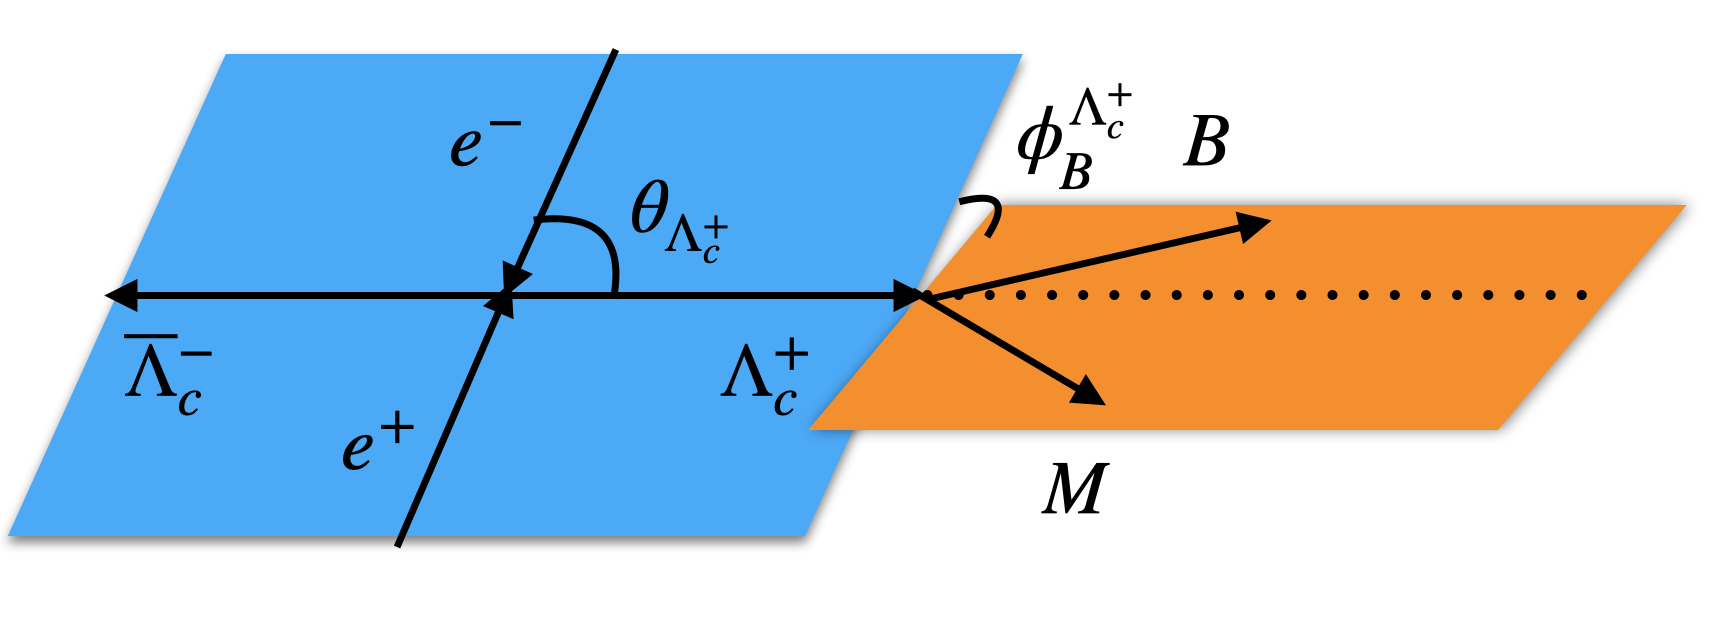
\includegraphics[width=0.50\textwidth]{figure/helicity.png}
    \caption{Definition of helicity angle in the process of $e^+e^- \to \lcp\lcm$ and $\lcp \to BM$. $B$ and $M$ denotes baryon and meson in the decay of $\lcp$. $\theta_{\lcp}$ is the angle between the $\lcp$ and $e^+e^-$ in the rest frame of $e^+e^-$. $\phi_{B}^{\lcp}$ is the angle between the production plane of $\lcp$ and plane determined by the decay products of $\lcp$.} 
    \label{fig:helicity_ee_lclp}
\end{figure}

In this analysis, we perform a amplitude analysis for $e^+e^- \to \lcp\lcm$, $\lcp \to p K^- \pi^+$ and $\lcm$ decays inclusively, using data samples collected at thirteen center-of-mass energies from 4.600 to 4.951 GeV with the BESSIII detector at BEPCII. The charge conjugation is always implied. The transverse polarization parameters, $\alpha_0$ and $\sin\Delta_0$ are obtained at each energy points. Based on the amplitude analysis results of $\lcp \to pK^-\pi^+$, the composition of the resonance structures are obtained in the $pK^-\pi^+$ final state. The decay asymmetry parameters of quasi-two-body $\lcp$ decay are also provided.
